\documentclass[journal]{new-aiaa}
\usepackage[utf8]{inputenc}
\usepackage{graphicx,amsmath,longtable,tabularx,booktabs,placeins}
\renewcommand{\topfraction}{0.9}
\renewcommand{\bottomfraction}{0.8}
\renewcommand{\textfraction}{0.08}
\renewcommand{\floatpagefraction}{0.78}
\setcounter{topnumber}{3}
\setcounter{bottomnumber}{2}
\setcounter{totalnumber}{4}
\setlength\LTleft{0pt}
\newcommand{\CM}{C_M^A}
\newcommand{\degc}{^\circ}
% Primitive input keeps table rows expandable before booktabs rules.
\makeatletter
\newcommand{\tablerows}[1]{\@@input #1.tex }
\makeatother
\title{Pre-Stall Load Redistribution on Swept Tailplane Models with Full-Span Controls}
\author{Andrea Rausa\footnote{PhD, Department of Aerospace Science and Technology, Corresponding Author, andrea.rausa@polimi.it},
Alex Zanotti\footnote{Associate Professor, Department of Aerospace Science and Technology}, Giuseppe Gibertini\footnote{Associate Professor, Department of Aerospace Science and Technology}, Alberto Guardone\footnote{Full Professor, Department of Aerospace Science and Technology}, and Franco Auteri\footnote{Full Professor, Department of Aerospace Science and Technology}}
\affil{Politecnico di Milano, Department of Aerospace Science and Technology, Milano, Italy, 20154}
\usepackage{lineno}
\begin{document}
\linenumbers
\maketitle
\begin{abstract}
\label{anchor:abstract}
Wind-tunnel measurements on swept tailplane models with deflected full-span controls show that lift growth can slow and then recover well before stall, with accompanying changes in pitching moment. Reynolds-averaged Navier--Stokes calculations reproduce the reduction in lift growth on the aft-swept reference model at a higher incidence than measured. The computed loads explain how total lift can continue to rise through this interval. The control loses lift while the fixed surface still gains lift, though more slowly than its preceding trend predicts. The fixed surface thus accounts for most of the shortfall in lift growth, while the control contributes most of the pitching-moment departure in the reference load breakdown. Lift growth subsequently recovers even as reverse flow spreads over the control. Comparisons across dihedral and sweep angles examine how tailplane geometry affects the incidence range and character of these pre-stall nonlinearities.
\end{abstract}

\section*{Nomenclature}
\begin{longtable*}{@{}l@{\quad=\quad}>{\raggedright\arraybackslash}p{.77\linewidth}@{}}
$C_D,C_L$ & drag and lift coefficients \\
$C_{F,k}$ & body-force coefficient, $k=x,y,z$ \\
$C_M^A,C_M^O,C_M^{A_I}$ & pitching-moment coefficients about the aerodynamic center, origin, or common axis \\
$C_p,\ \mathbf C_f,C_{f,c}$ & pressure, vector skin-friction, and chordwise skin-friction coefficients \\
$D_{Q,j}$ & departure from the preceding coefficient trend \\
$F_k$ & body-force component, N \\
$\mathcal I_M$ & difference in moment increments between dihedral cases \\
$M_\infty$ & freestream Mach number \\
$Q$ & coefficient label, $L$ or $M$ \\
$Re_b,Re_{\bar c}$ & semispan and mean-chord Reynolds numbers \\
$S$ & reference semiplanform area, m$^2$ \\
$T_\infty$ & freestream temperature, K \\
$U_\infty$ & freestream speed, m/s \\
$b$ & geometric semispan, m \\
$c,\ \bar c$ & local and mean aerodynamic chords, m \\
$f_{\mathrm{rev}}$ & upper control surface area fraction with reverse flow \\
$i,j,k$ & sample, surface-contribution, and force-component indices \\
$m_{Q,j}^{\mathrm{pre}}$ & preceding slope, per degree \\
$p,p_\infty$ & surface and freestream pressures, Pa \\
$q_\infty$ & freestream dynamic pressure, Pa \\
$s$ & spanwise coordinate, m \\
$t$ & section thickness, m \\
$\mathbf t_c$ & downstream chordwise unit tangent \\
$u_i,w_i$ & supplied sample uncertainty magnitude and linear-combination weight \\
$u_{\mathrm{ind}},u_{\mathrm{L1}}$ & uncertainty sensitivities for coefficient departures \\
$x,y,z$ & downstream, spanwise, and upward body coordinates, m \\
$y^+$ & nondimensional wall distance \\
$x_A,x_O$ & streamwise coordinates of the aerodynamic center and origin, m \\
$\alpha,\alpha_a,\alpha_b$ & incidence and interval endpoints, deg \\
$\Gamma,\delta$ & dihedral and control deflection, deg \\
$\Delta C_{Q,j}$ & actual coefficient increment \\
$\eta=s/b,\ \xi$ & span fraction and chord fraction with control deflection removed \\
$\lambda,\Lambda$ & quarter-chord sweep (deg) and aspect ratio \\
$\rho_\infty$ & freestream density, kg/m$^3$ \\
$\tau,\boldsymbol\tau_w$ & taper ratio and wall-shear vector (Pa) \\
\end{longtable*}
% The unnumbered nomenclature must not consume a numbered-table entry.
\setcounter{table}{0}

\section{Introduction}\label{sec:intro}
The lift-curve slope of a swept tailplane with a deflected trailing-edge control can decrease over a narrow incidence range and then recover well before stall. Control deflection affects where and how much the slope decreases. The pitching-moment coefficient can depart from its preceding trend over a different interval. These localized changes motivate an examination of how the loads on the fixed surface and the control evolve with incidence.

Plain-flap experiments by Sears and Liddell~\cite{sears1942plain} documented reduced flap effectiveness associated with separation at large deflections. Their hinge-moment measurements showed that similar changes in lift can load the flap differently. For finite rectangular wings with full-span flaps, Campbell et al.~\cite{campbell1956fullspan} showed how flap chord and aspect ratio affect both lift and the location of the center of pressure.

On swept wings, changes in loading can give rise to pitching-moment nonlinearity before maximum lift~\cite{harper1964sweptstall}. The lift coefficient reflects the integrated lift, whereas the pitching-moment coefficient also depends on where the forces act relative to the reference axis. The two coefficients therefore provide complementary evidence about pre-stall loading changes.

Experiments on swept wings with flaps also show that separated flow can coexist with increasing total lift. Tewes et al.~\cite{tewes2014sweepcontrol} found that large deflection could produce separated flap flow with continued lift growth, while sweep altered the associated lift and pitching-moment response. Melton~\cite{melton2014sweptflap} observed spanwise variation in separated flow on a swept wing with a 30\%-chord flap. Toppings and Yarusevych~\cite{toppings2021wingtip} also documented spanwise variation in a separation bubble near the tip of an unswept wing. The swept-flap experiments primarily investigated active separation control and cannot quantitatively validate the present configurations. They provide context for interpreting the present lift and moment trends.

The MONNALISA database study~\cite{rausa2026monnalisa} documented pre-stall lift nonlinearity, reverse flow on the control, associated pressure changes, and continued total lift growth.

For longitudinal static stability, the relevant quantity is the local slope of pitching moment with incidence near trim. If the tailplane operates in a nonlinear range, a numerical model must capture the changes in that slope to estimate the tailplane's contribution to stability.

We investigate where lift growth slows and recovers before stall and how pitching moment changes over the same range. We examine the effects of control deflection, tailplane planform, and dihedral. We compare Reynolds-averaged Navier--Stokes (RANS) predictions with wind-tunnel measurements of the integrated loads. We then use the computed pressure and wall shear to identify the contributions of the fixed surface and control.

\label{end:sec:intro}
\section{Methodology}\label{sec:methods}
\subsection{Models and wind-tunnel setup}\label{sec:setup}
We tested two isolated tailplane-inspired wings in the wind tunnel (WT), without a fuselage or a main-wing wake. Configuration I is aft-swept and was tested at $\Gamma=0\degc$ and $45\degc$. Configuration II is forward-swept and was tested at zero dihedral.

Both wings use the same symmetric section with thickness ratio $t/c=9\%$, geometric semispan $b=1.6$~m, and a full-span plain control hinged at 70\% chord. Table~\ref{tab:geometry} gives the reference semiplanform area and mean aerodynamic chord for each model. Model I uses the same values at both dihedral settings. Model I has $+30\degc$ quarter-chord sweep and model II has $-15\degc$. Positive dihedral raises the tip, and the full-wing aspect ratio is $\Lambda=2b^2/S$.

\begin{table}[htbp]\centering
\caption{Model geometry and coefficient reference quantities.}\label{tab:geometry}
\begin{tabular}{lccc}\toprule
Property & I, $\Gamma=0\degc$ & I, $\Gamma=45\degc$ & II, $\Gamma=0\degc$ \\\midrule
$\lambda$ (deg) & 30 & 30 & $-15$ \\
$\Lambda$ & 5.0 & 5.0 & 5.2 \\
$\tau$ & 0.4 & 0.4 & 0.6 \\
$S$ (m$^2$) & 1.024 & 1.024 & 0.984604 \\
$\bar c$ (m) & 0.679184 & 0.679184 & 0.6282 \\
Root chord (m, rounded) & 0.914286 & 0.914286 & 0.76923 \\
$Re_{\bar c}$ & $2.335\times10^6$ & $2.335\times10^6$ & $2.159\times10^6$ \\
Numerical $x_A$ (m) & 0.642000 & 0.643532 & $-0.003618$ \\\bottomrule
\end{tabular}
\end{table}

\begin{figure}[htbp]\centering
\begin{minipage}[c]{.30\textwidth}\centering
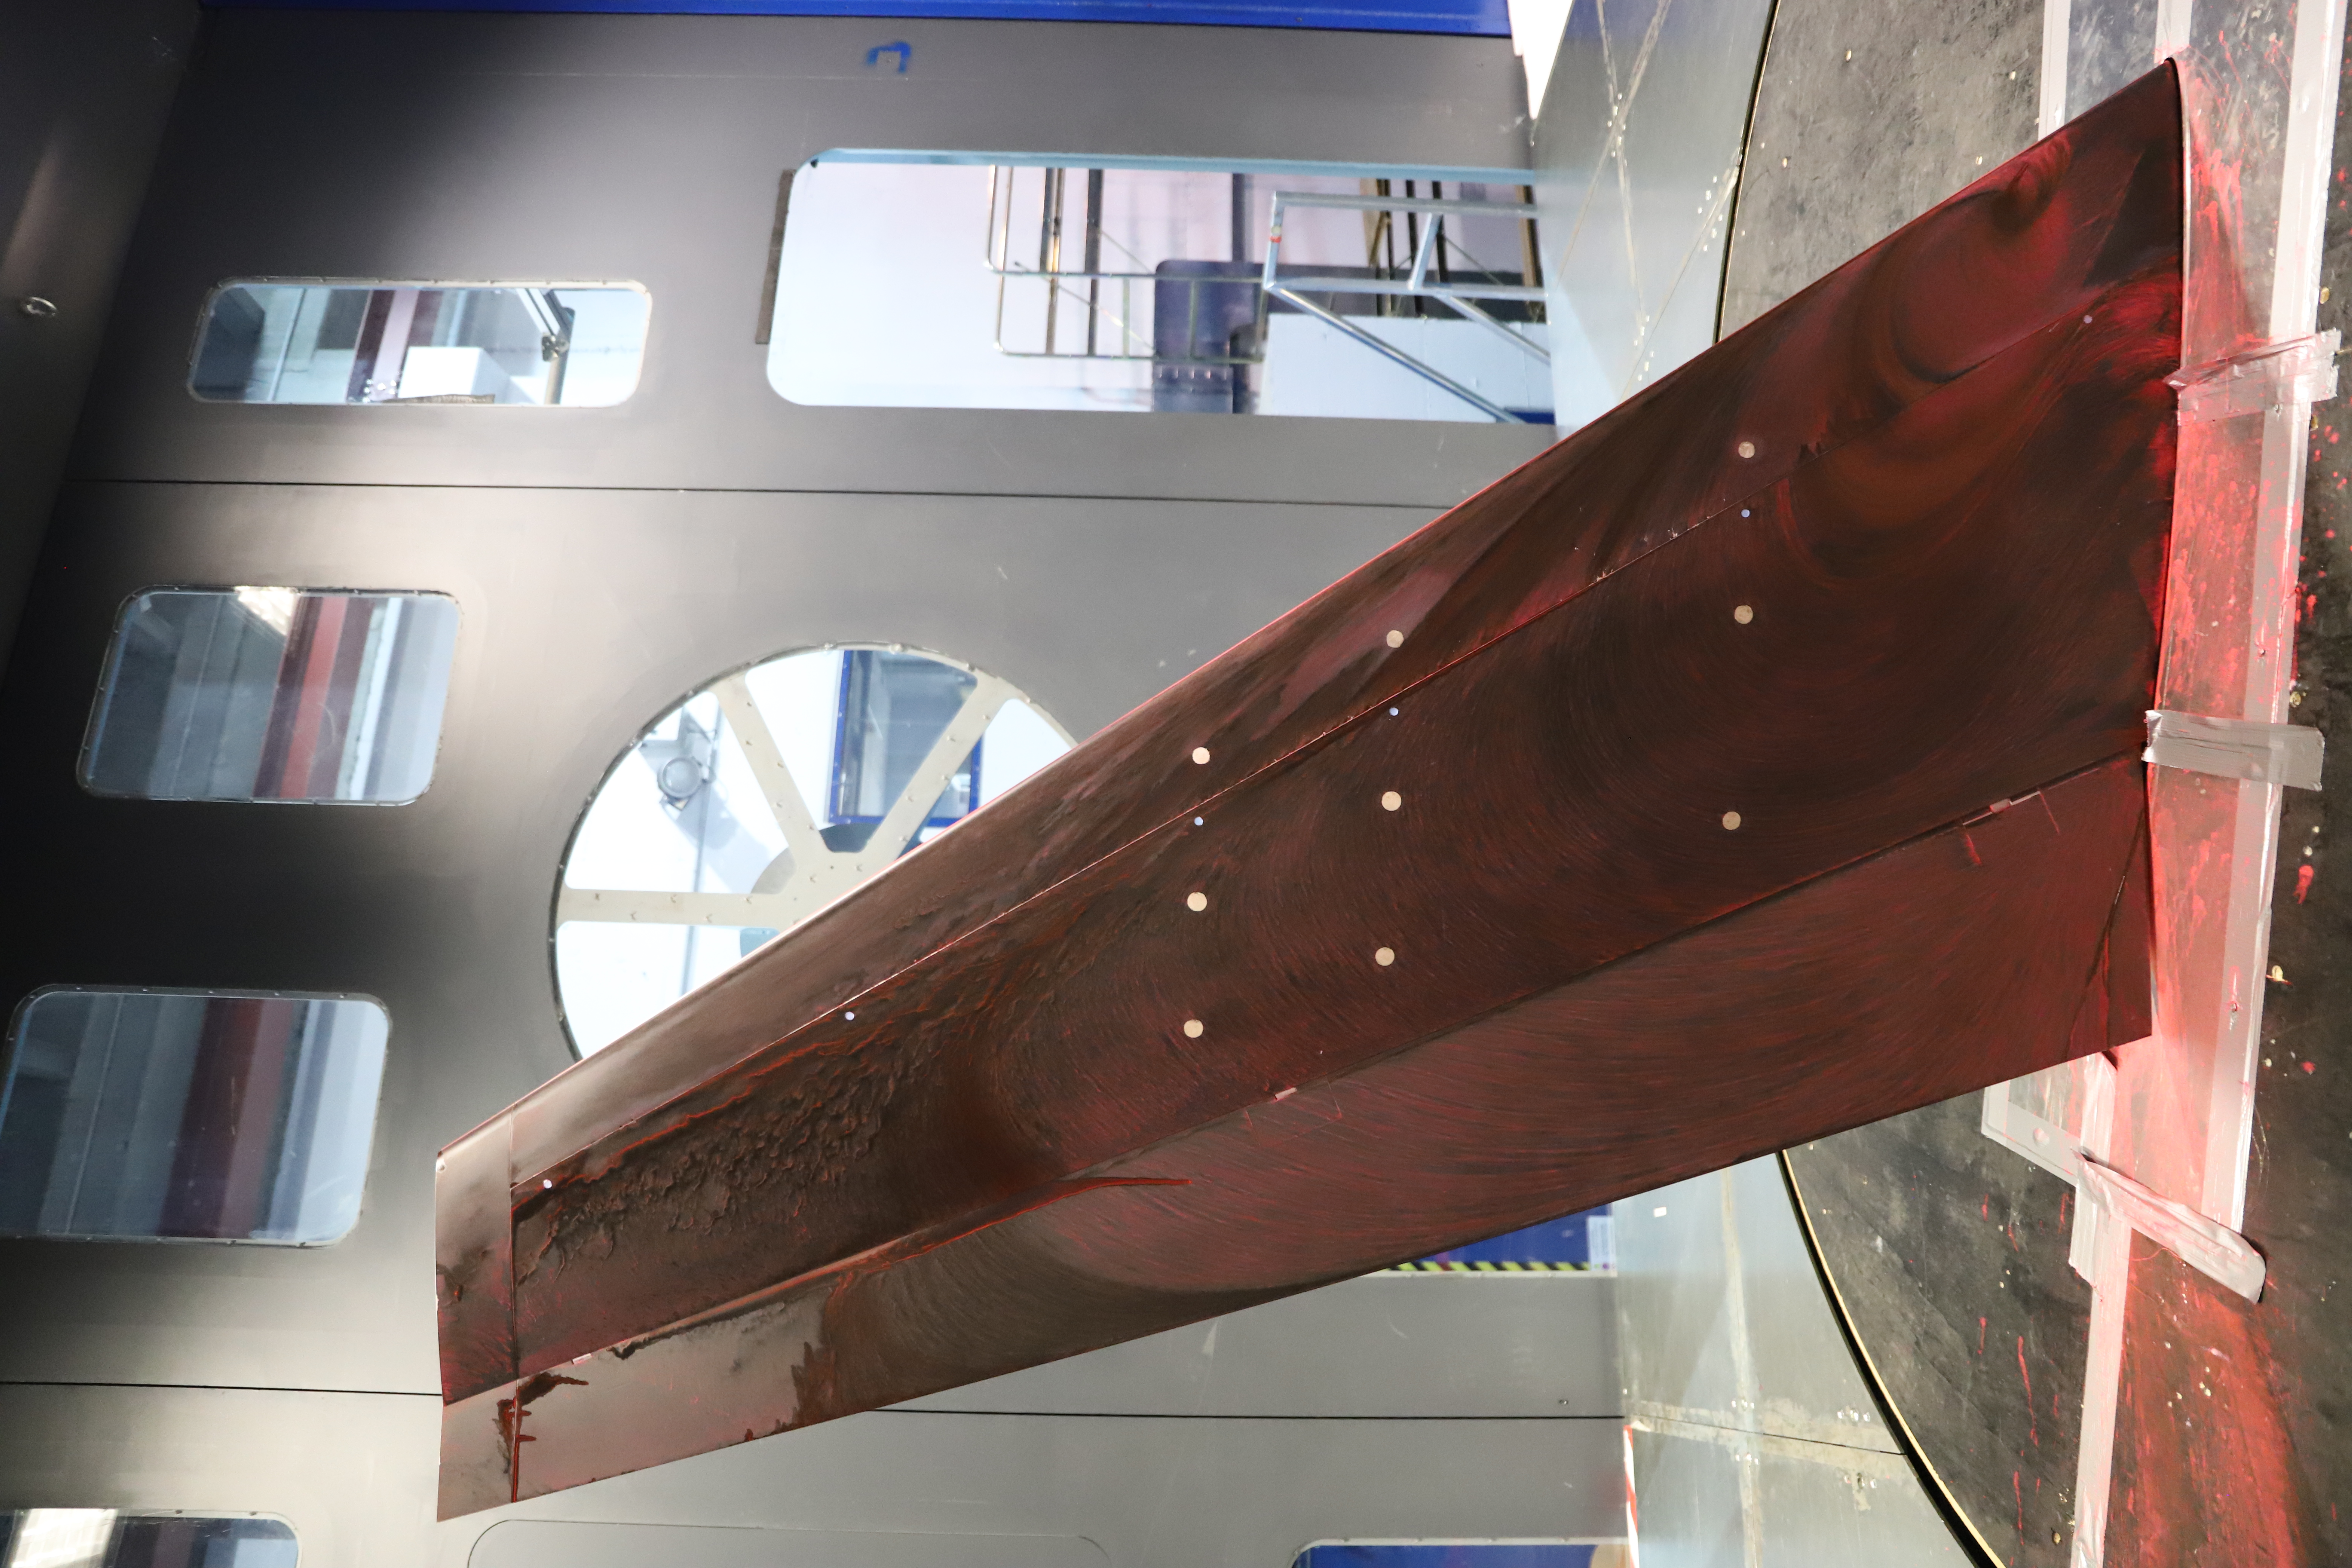
\includegraphics[angle=-90,origin=c,width=\linewidth]{figures_revision_installation.JPG}\\(a)
\end{minipage}\hfill
\begin{minipage}[c]{.65\textwidth}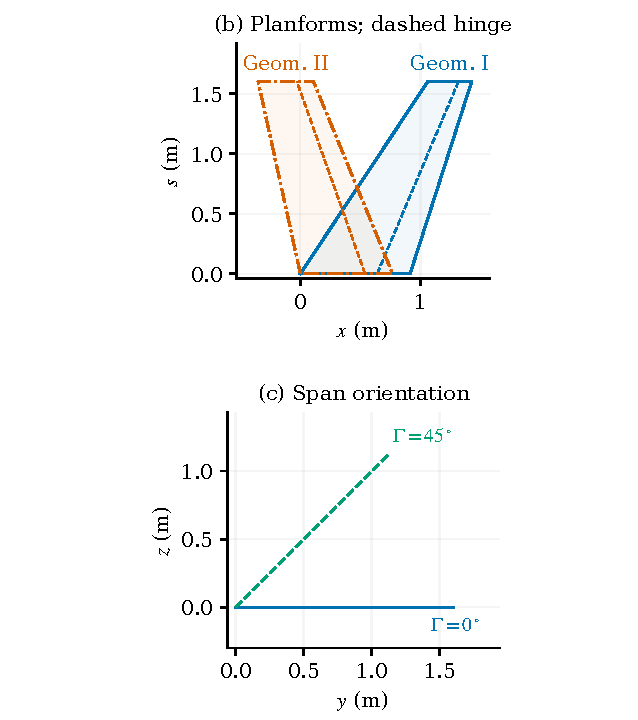
\includegraphics[width=\linewidth]{figures_revision_geometry.pdf}\end{minipage}
\caption{(a) Wind-tunnel installation, (b) reference and forward-swept planforms, and (c) zero- and positive-dihedral configurations.}\label{fig:setup}
\end{figure}

Measurements were obtained in the closed-circuit wind tunnel at Politecnico di Milano. Figure~\ref{fig:setup}a shows the mounted model at $\alpha=25\degc$ and $\delta=20\degc$. The test section is 4.00~m wide and 6.00~m long. A raised floor reduced its height from 3.84 to 3.49~m. The model semispan is 40\% of the tunnel width. The inlet and gap beneath the raised floor were designed to divert the incoming floor boundary layer under the model.

The database~\cite{rausa2026monnalisa} reports freestream turbulence below 0.1\%. Outside the wind-tunnel wall boundary layers, total-pressure variations stay within $\pm0.5\%$ of dynamic pressure over most of the section and within $\pm1\%$ overall. The longitudinal static-pressure gradient is $\partial C_P/\partial x=-0.004$~m$^{-1}$. A RUAG 767 strain-gauge balance and HBM QuantumX system supplied the forces and moments. The nominal operating point was $M_\infty=0.147$, $T_\infty=300$~K, and semispan-based $Re_b=5.5\times10^6$. Table~\ref{tab:geometry} reports chord-based Reynolds numbers, obtained from $Re_{\bar c}=Re_b\bar c/b$.

\label{anchor:wt_uncertainty}Incidence ranged from approximately $-25\degc$ to $25\degc$, with $2\degc$ spacing near the pre-stall changes. Control deflections were $\delta=0,10,20,30\degc$. The error bars show the supplied propagated uncertainties, which include the strain-gauge balance and the transformation to wind axes. Moment uncertainties correspond to moments about the fitted aerodynamic centers. These magnitudes also underpin the departure sensitivity analysis in Sec.~\ref{sec:analysis}.

\label{end:sec:setup}
\subsection{Conventions and moment references}\label{sec:references}
Positive incidence raises the leading edge, positive control deflection moves the trailing edge downward, and positive pitching moment is nose-up. Body axes are downstream ($x$), spanwise ($y$), and upward ($z$). Forces are normalized by $q_\infty S$; lift and drag follow from the body-axis components:
\begin{equation}
 C_L=C_{F,z}\cos\alpha-C_{F,x}\sin\alpha,\qquad
 C_D=C_{F,z}\sin\alpha+C_{F,x}\cos\alpha,\qquad
 C_{F,k}=F_k/(q_\infty S).
\label{eq:force}
\end{equation}
Pitching moment is normalized by $q_\infty S\bar c$. Body coordinates are expressed relative to the root leading edge.

\label{anchor:fitted_reference}We obtained separate wind-tunnel and RANS aerodynamic centers by fitting pitching moment and body-normal force at zero control deflection over $|\alpha|\leq10\degc$~\cite{rausa2026monnalisa}. Each center remains fixed as control deflection changes. Measured and computed positions are 0.6430 and 0.6420~m at zero dihedral and 0.6455 and 0.6435~m at $45\degc$ for model I. They differ by about 1 and 2~mm, respectively. For model II, the positions are $-0.0492$ and $-0.00362$~m, a difference of 45.6~mm. The WT--RANS curves use the respective fitted references.

The original numerical reference is $O=(0.228571,0,0)$~m, at the root quarter-chord of model I. To move the moment reference from $x_0$ to $x_1$, we add the moment of the body-axis force $F_z$ over that distance
\begin{equation}
 C_M(x_1)=C_M(x_0)+\frac{x_1-x_0}{\bar c}C_{F,z}.
\label{eq:transport}
\end{equation}
Table~\ref{tab:geometry} lists the computed aerodynamic centers and the area and chord used to normalize the coefficients. We compare the computed moment changes at both dihedral settings about $A_I=(0.642000,0,0)$~m. This is the computed aerodynamic center of model I at zero dihedral. We denote the resulting moment coefficient by $C_M^{A_I}$.

\label{end:sec:references}
\subsection{Numerical setup}\label{sec:numerics}
SU2~\cite{palacios2013stanford} solves compressible ideal-gas RANS with Sutherland viscosity, Spalart--Allmaras turbulence~\cite{spalart1992sa}, and the Bas--Cakmakcioglu transition model~\cite{cakmakcioglu2020bcm}. The mean-flow equations use vertex-centered median-dual cells, Roe fluxes and second-order MUSCL reconstruction~\cite{van1979towards}, Green--Gauss gradients and a Venkatakrishnan limiter~\cite{venkatakrishnan1993accuracy} (coefficient 0.05). The turbulence equation uses first-order upwinding for convection.

\label{anchor:wall_model}The wing has no-slip, adiabatic surfaces. The far field uses freestream conditions, and the root symmetry plane omits the model support and the boundary layer over the raised floor. The steady calculation uses implicit Euler pseudo-time stepping with a flexible generalized minimal residual (FGMRES) solver and an adaptive Courant--Friedrichs--Lewy (CFL) number. The convergence check uses a Cauchy criterion on lift and drag over 100 samples, with a typical tolerance of $3\times10^{-6}$.

Hex-dominant, octree-based meshes~\cite{rausa2026monnalisa} resolve the leading edge, hinge junction, trailing edge, and incidence-dependent wake. Boundary-layer extrusion has nominal first-cell height $2\times10^{-6}$~m and growth ratio 1.15. Representative median wall distance is $y^+=0.19$--0.26, with maxima 1.1--1.3.

A four-level grid study on configuration I used $\delta=35\degc$, $\Gamma=0,45\degc$ and $\alpha=0,18\degc$ (Table~\ref{tab:mesh}, Fig.~\ref{fig:mesh}). Nominal meshes had 9.7--12.7 million points versus 50.1--65.9 million on the finest level. Moments in Fig.~\ref{fig:mesh} use the original numerical pole.

Nominal-to-finest differences were 1.20--2.14\% in lift and 1.13--2.49\% in drag. At $\Gamma=0\degc$, $\alpha=18\degc$, $C_M^O$ changed from $-0.813$ to $-0.827$; the $45\degc$ moment sequence was nonmonotonic. We used nominal meshes to limit the computational cost of the full case set. The refinement study quantifies grid sensitivity for integrated lift, drag and pitching moment. The individual surface contributions were evaluated on the nominal meshes.

\begin{table}[htbp]\centering
\caption{Point and volume-element ranges, in millions, for the four-level refinement assessment.}\label{tab:mesh}
\begin{tabular}{lrr}\toprule
Refinement & Points & Volume elements \\\midrule
Coarse & 4.79--5.29 & 9.51--10.90 \\
Nominal & 9.67--12.74 & 19.06--24.07 \\
Fine & 22.33--26.56 & 39.93--45.70 \\
Very fine & 50.11--65.89 & 87.35--109.98 \\
\bottomrule\end{tabular}\end{table}

\begin{figure}[htbp]\centering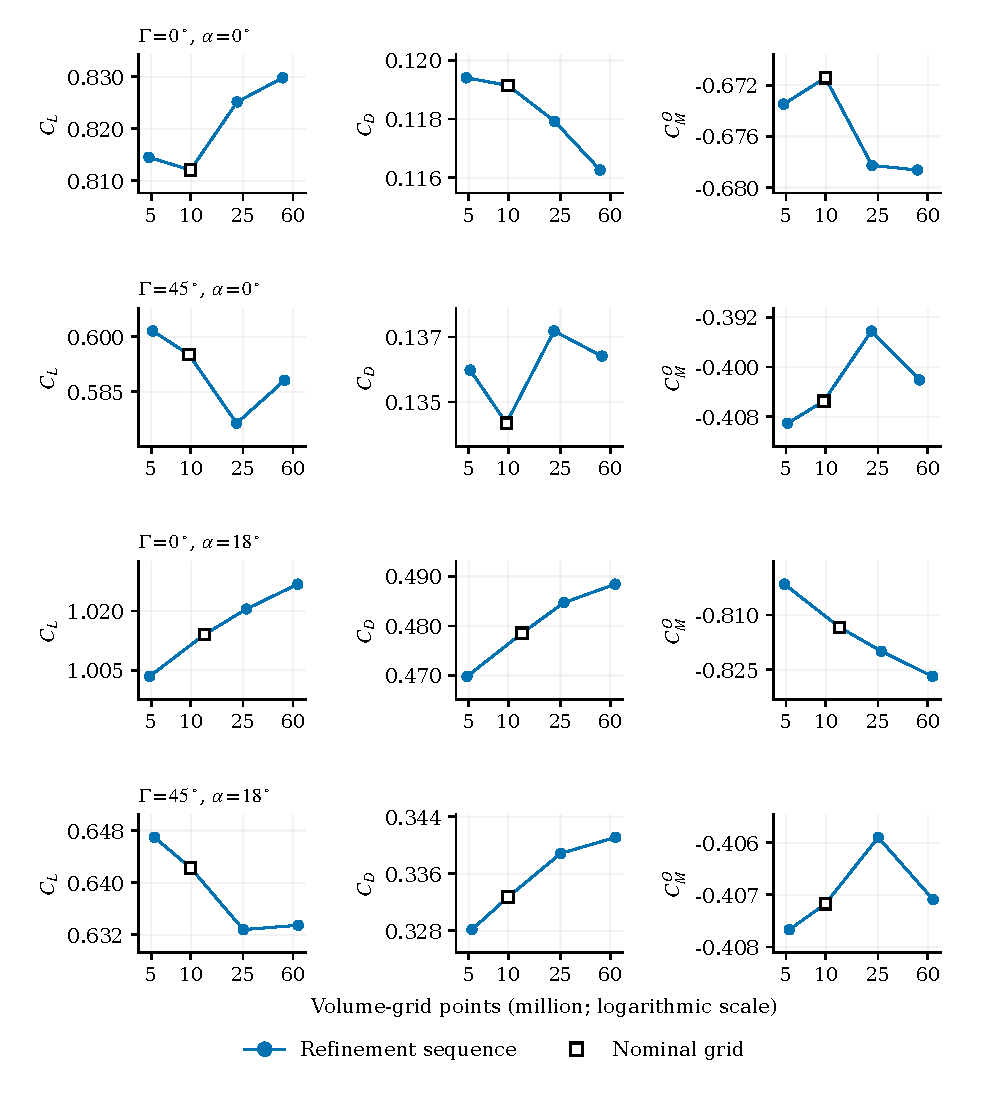
\includegraphics[width=\textwidth]{figures_revision_mesh_refinement.pdf}
\caption{Grid-refinement trends of lift, drag, and pitching moment for configuration I at $\delta=35\degc$, two incidences, and two dihedral settings.}\label{fig:mesh}\end{figure}

\label{end:sec:numerics}
\subsection{Load decomposition and trend departures}\label{sec:analysis}
When lift growth slows, the lift coefficient can still increase. We compare the lift gain between two sampled angles with the gain expected from the preceding trend. We use the same procedure for pitching moment.

For lift or pitching moment (indexed by $Q$), the increment $\Delta C_{Q,j}$ and the departure $D_{Q,j}$ for the total or for component $j$ are
\begin{equation}
 \Delta C_{Q,j}=C_{Q,j}(\alpha_b)-C_{Q,j}(\alpha_a),\qquad
 D_{Q,j}=\Delta C_{Q,j}-m_{Q,j}^{\mathrm{pre}}(\alpha_b-\alpha_a).
\label{eq:departure}
\end{equation}
For example, from $\alpha=0\degc$ to $2\degc$ at $\delta=20\degc$, the computed fixed-surface lift coefficient rises by 0.0593. Continuing the earlier slope over that interval would give a rise of 0.1285. The lift gain is therefore 0.0692 smaller, giving a departure of $-0.0692$.

We fit the preceding slope by unweighted least squares. Using the same fit samples for all components in a comparison ensures that their departures sum to the total. For the reference RANS model, the primary fits use $\alpha\in\{-6,-4,-2\}\degc$ at $\delta=20\degc$ and $\{-16,-14,-12\}\degc$ for the early change at $\delta=30\degc$. The incidence samples used to fit the wind-tunnel trends are given with the corresponding results. These slopes summarize the data before each interval without assuming a flow state. Appendix~\ref{app:sensitivity} shows how the departures in the reference calculation at $20\degc$ deflection vary with the fitting range. The other fit comparisons are discussed with the corresponding results.

To judge the measured departures against the measurement uncertainty, we express each departure as $D=\sum_i w_i C_i$. The weights account for both the interval endpoints and the samples used to fit the preceding trend. We propagate the supplied uncertainties for these samples into two estimates.
\begin{equation}
 u_{\mathrm{ind}}=\left[\sum_i(w_i u_i)^2\right]^{1/2},\qquad
 u_{\mathrm{L1}}=\sum_i|w_i|u_i.
\label{eq:uncertainty}
\end{equation}
The first estimate assumes independent errors across the samples. The second gives the largest possible error in the departure if every sample error stays within its supplied magnitude. The supplied uncertainties give neither the error correlations between angles nor a confidence level for the departure.

To identify which surfaces produce the computed departures, we integrate the pressure and wall-shear forces over the fixed surface, control, and tip using common reference quantities for each model. The control includes the hinge junction and blunt trailing edge. Tip loads are included in the totals.

The pressure and wall-shear forces are integrated over the triangulated surface. The pressure coefficient is $C_p=(p-p_\infty)/q_\infty$ and wall-shear coefficient $\mathbf C_f=\boldsymbol\tau_w/q_\infty$. The moment about reference abscissa $x_A$ is
\begin{equation}
 C_M(x_A)=\frac{1}{q_\infty S\bar c}
 \int\big[z\,dF_x-(x-x_A)dF_z\big].
\label{eq:moment}
\end{equation}
We retain the moments of the axial force, $z\,dF_x$, and the upward force, $-(x-x_A)dF_z$, separately for the dihedral comparison about a common axis. The integrated surface forces and moments agree with the solver totals.

The surface totals show which component contributes to the departure. Dividing each surface into smaller regions shows where the loads change. The position of those regions relative to the pitch axis helps explain their contribution to pitching moment. We define $\xi$ as the local chord fraction after rotating the control back to zero deflection. The chordwise regions are forward ($\xi<0.4$), intermediate ($0.4\leq\xi<0.7$), and aft ($\xi\geq0.7$). The aft region is further divided into spanwise thirds, using $\eta=s/b$ (Fig.~\ref{fig:regions}). Integrals cover both physical sides, with hinge junction and end-face loads included in the appropriate totals. To relate the regional loads to changes in suction near the leading edge and hinge, we also use pressure cuts. The cuts at $\eta=0.2,0.5,0.8$ follow the actual surface intersections without smoothing or bridging gaps. The regional coefficients are integrals over the corresponding regions.

\begin{figure}[htbp]\centering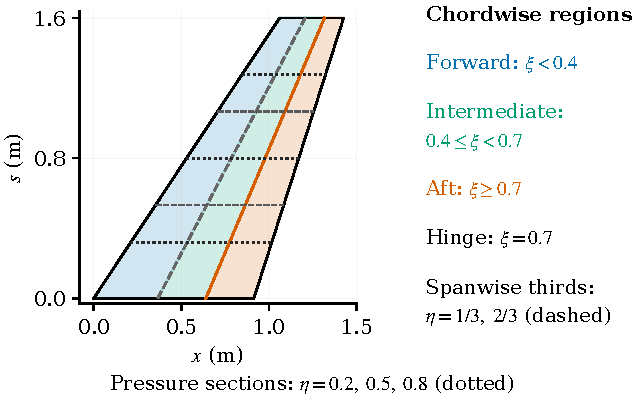
\includegraphics[width=.72\textwidth]{figures_revision_load_regions.pdf}
\caption{Reference planform: chordwise loading regions, spanwise thirds, hinge, and pressure-section locations.}\label{fig:regions}\end{figure}

\label{anchor:reversal_definition}We use the direction of wall shear to track where reverse flow occurs on the control and how much area it covers. On each surface face, we project the downstream chord direction $\mathbf d_c$ onto the face and normalize it to obtain a unit tangent. On the control, $\mathbf d_c$ follows the deflected chord. For a face with unit normal $\mathbf n$, the tangent is $\mathbf t_c=[\mathbf d_c-(\mathbf d_c\cdot\mathbf n)\mathbf n]/\|\mathbf d_c-(\mathbf d_c\cdot\mathbf n)\mathbf n\|$. The coefficient $C_{f,c}=\mathbf C_f\cdot\mathbf t_c$ is the component of the skin-friction coefficient along that tangent.

The reverse-flow area fraction $f_{\mathrm{rev}}$ is the fraction of the upper control surface ($\xi>0.7$, excluding end faces) where $C_{f,c}<0$. This fraction measures the extent of upstream-directed chordwise wall shear and can be compared across the intervals of slower and recovering lift growth. Identifying the full three-dimensional separation pattern requires more information about the surface flow~\cite{tobak1982topology,mccormack1949sweptforward}.

\label{end:sec:analysis}
\label{end:sec:methods}
\section{Experimental--Numerical Comparison}\label{sec:response}
Figure~\ref{fig:measured} shows how the reference lift and pitching-moment curves depart from their lower-incidence trends as control deflection increases. The lift curve can steepen again before stall, and the moment response can change over a different incidence interval.

\begin{figure}[htbp]\centering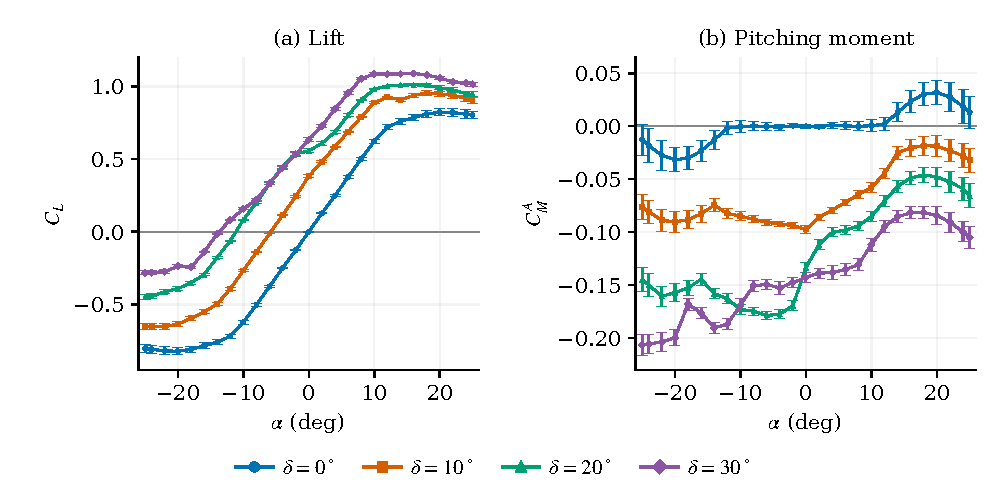
\includegraphics[width=\textwidth]{figures_revision_measured_baseline.pdf}
\caption{Reference wind-tunnel lift and moment at zero dihedral. Bars show propagated pointwise uncertainty.}\label{fig:measured}\end{figure}

\label{anchor:uncertainty}For configuration I at $\delta=20\degc$, the measured lift coefficient rises by 0.089 from $\alpha=-4\degc$ to $-2\degc$, then by only 0.020 from $-2\degc$ to $0\degc$. Over the latter interval, the pitching-moment coefficient about the experimental aerodynamic center increases by 0.036. We fit the preceding trends at $\alpha\in\{-6,-4,-2\}\degc$. Both coefficients depart from those trends by more than either uncertainty estimate (Table~\ref{tab:wt}). The supplied uncertainties in the individual lift and moment values are approximately 0.013 and 0.0046--0.0047, respectively.

\begin{table}[htbp]\centering\small
\caption{Measured lift and moment departures and uncertainty sensitivities for the reference configuration at $\delta=20\degc$}\label{tab:wt}
\begin{tabular}{llrrrr}\toprule
Geom., $\Gamma$, $\delta$ & Coefficient & $\alpha$ interval (deg) & $D$ & $u_{\mathrm{ind}}$ & $u_{\mathrm{L1}}$ \\\midrule
\tablerows{tables_revision_wt_reference_rows}
\bottomrule\end{tabular}\end{table}

At $\delta=10\degc$, the measured moment coefficient falls by 0.0038 from $\alpha=-2\degc$ to $0\degc$ and rises by 0.011 from $0\degc$ to $2\degc$. The pronounced reduction in lift growth occurs at the higher deflection of $20\degc$. At $\delta=30\degc$, lift grows more slowly at lower incidence. The lift coefficient increases by 0.077 from $\alpha=-12\degc$ to $-10\degc$ and by 0.064 from $-10\degc$ to $-8\degc$, before the increase rises to 0.111 over $-8\degc$ to $-6\degc$. The moment coefficient rises by about 0.018 in each of the first two intervals. The lift slope already varies at lower incidences, which makes a departure based on a straight-line fit sensitive to the chosen samples.

\FloatBarrier
\label{anchor:comparison}Figure~\ref{fig:comparison} compares WT (filled symbols, solid lines) with RANS (open symbols, dashed lines); circles and squares distinguish $\delta=20\degc$ and $30\degc$. Plain and hatched grey bands mark selected measured incidence intervals at $\delta=20\degc$ and $30\degc$, respectively. Moments use each dataset's aerodynamic center.

\begin{figure}[htbp]\centering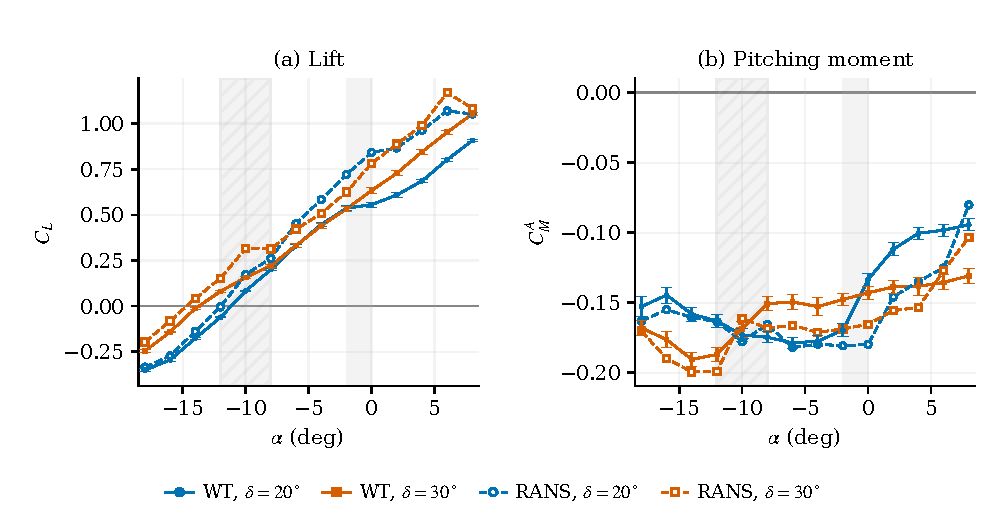
\includegraphics[width=\textwidth]{figures_revision_comparison.pdf}
\caption{Reference WT and RANS lift and pitching moment. Error bars show propagated WT uncertainties.}\label{fig:comparison}\end{figure}

At $\delta=20\degc$ and zero incidence, the computed lift coefficient is about 0.842, and the measured value is 0.556, with a measurement uncertainty of 0.013. At $\delta=30\degc$, the change in lift slope is sharper in RANS than in the measurements. The computed moment departure at this deflection also depends strongly on which earlier angles are fitted.

At $20\degc$ deflection, both datasets show slower lift growth accompanied by an increase in pitching-moment coefficient. The reduction in lift growth occurs from $-2\degc$ to $0\degc$ in the tunnel and from $0\degc$ to $2\degc$ in RANS. The following analysis uses the computed surface loads to explain the reduction and examines the pressure and wall-shear changes as lift growth recovers.
\FloatBarrier
\label{end:sec:response}
\section{Load Breakdown of the Reference Model}\label{sec:joint}
\subsection{Fixed-surface and control-surface loads}\label{sec:budget}
We first determine which surface accounts for the reduced growth of total lift and which contributes to the simultaneous pitching-moment departure. For the reference model at zero dihedral and $\delta=20\degc$, the dashed lines in Fig.~\ref{fig:budget} extend the fitted slopes from the computed values at zero incidence. The departure is the computed value at $\alpha=2\degc$ minus the end of the corresponding trend line. The lower panels show the increments and departures separately.

\begin{figure}[htbp]\centering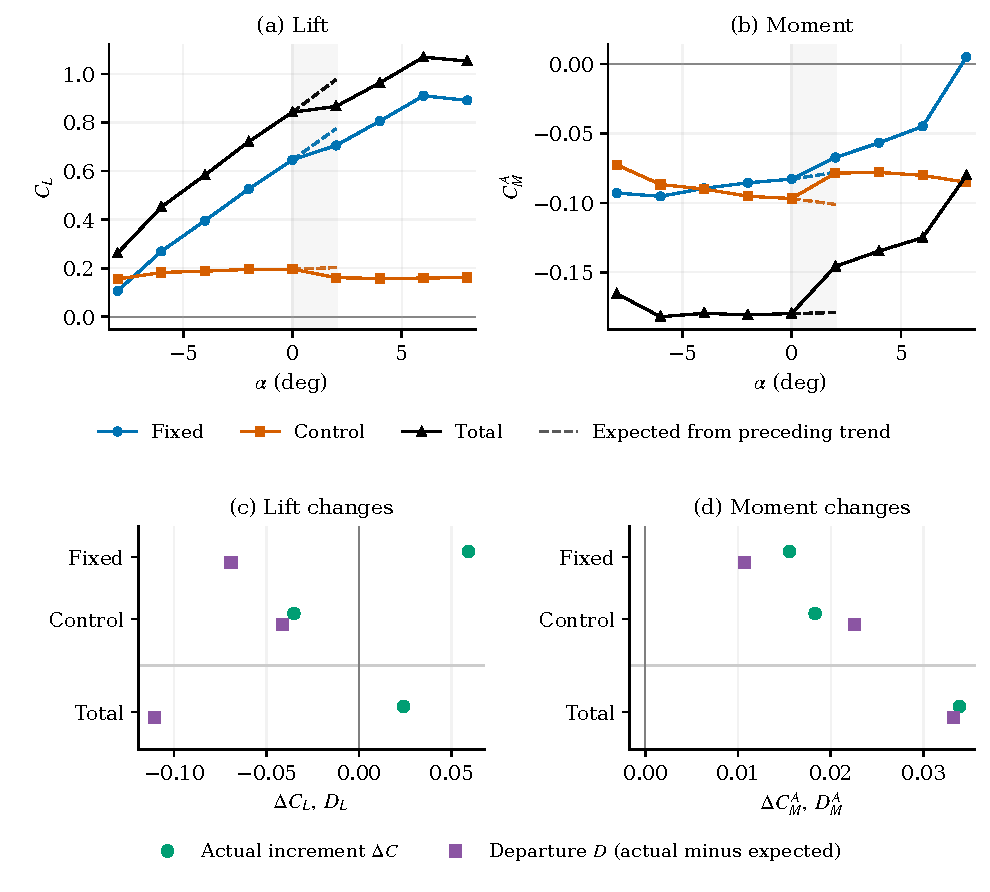
\includegraphics[width=\textwidth]{figures_revision_baseline_budget.pdf}
\caption{Fixed-surface, control-surface, and total numerical loading, with actual increments and departures from preceding incidence trends.}\label{fig:budget}\end{figure}

Over $\alpha=0\to2\degc$, the fixed-surface lift coefficient rises by 0.0593, and the control contribution falls by 0.0351. The total still rises by 0.0242. The fixed surface gains less lift than its earlier slope would suggest, and the control loses lift where its earlier slope would suggest a gain. Their departures are $-0.0692$ on the fixed surface and $-0.0414$ on the control, giving a total of $-0.1106$ (Table~\ref{tab:budget}). The tip contributes less than 0.09\% of the magnitude of each total departure in the table. The fixed surface therefore accounts for about 63\% of the shortfall in lift growth. Its share stays between 62.4\% and 62.6\% across the three fits in Appendix~\ref{app:sensitivity}, even though the total departure changes.

\begin{table}[htbp]\centering\small
\caption{Computed lift and moment departures for the reference configuration at zero dihedral}\label{tab:budget}
\begin{tabular}{llrrr}\toprule
Geom., $\delta$, $\alpha$ interval & Departure & Fixed & Control & Total \\\midrule
\tablerows{tables_revision_budget_rows_compact}
\bottomrule\end{tabular}\end{table}

We first evaluate the moments about the computed aerodynamic center. From $\alpha=0\degc$ to $2\degc$, the moment change on each surface is more positive than its earlier trend would suggest. The control contributes $+0.0226$ to the departure from that trend, and the fixed surface contributes $+0.0107$ (Table~\ref{tab:budget}). Which contribution is larger depends on the reference axis. About the original numerical origin, the fixed-surface and control departures are still positive, at $+0.0529$ and $+0.0474$, respectively.
\label{end:sec:budget}
\subsection{Pressure distribution and regional load changes}\label{sec:pressure}
Figure~\ref{fig:cp} compares the pressure distributions on both sides of the reference wing at three span stations for $\alpha=0\degc$ and $2\degc$. As incidence increases, suction strengthens near the leading edge and weakens near the hinge. Integrating the loads over the forward, intermediate and aft regions shows how these changes combine.

\begin{figure}[htbp]\centering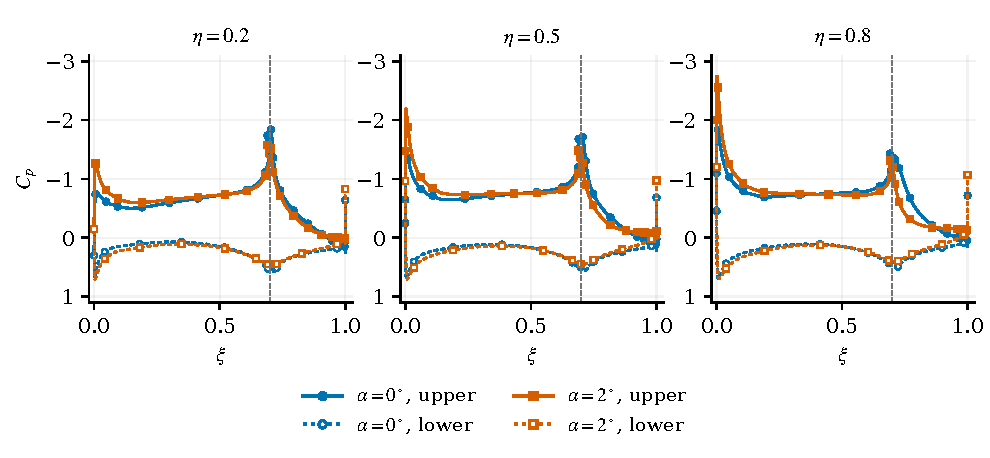
\includegraphics[width=\textwidth]{figures_revision_pressure_sections.pdf}
\caption{Chordwise pressure distributions at three span locations across the reference pre-stall loading change.}\label{fig:cp}\end{figure}

From $0\degc$ to $2\degc$ incidence, the integrated lift contribution of the forward region ($\xi<0.4$) rises by 0.0671. The earlier trend predicts a gain of 0.1027, giving a departure of $-0.0357$ using the unrounded values (Fig.~\ref{fig:spatial}a). In the intermediate region, the lift coefficient falls by 0.0097, compared with a predicted rise of 0.0257. Its departure is $-0.0354$.

The aft-region contribution falls by 0.0332. Continuing the earlier slope would give a gain of 0.0063, so the departure is $-0.0396$. Pressure forces account for nearly all of the lift-growth shortfall. The totals include the viscous contribution.

\begin{figure}[htbp]\centering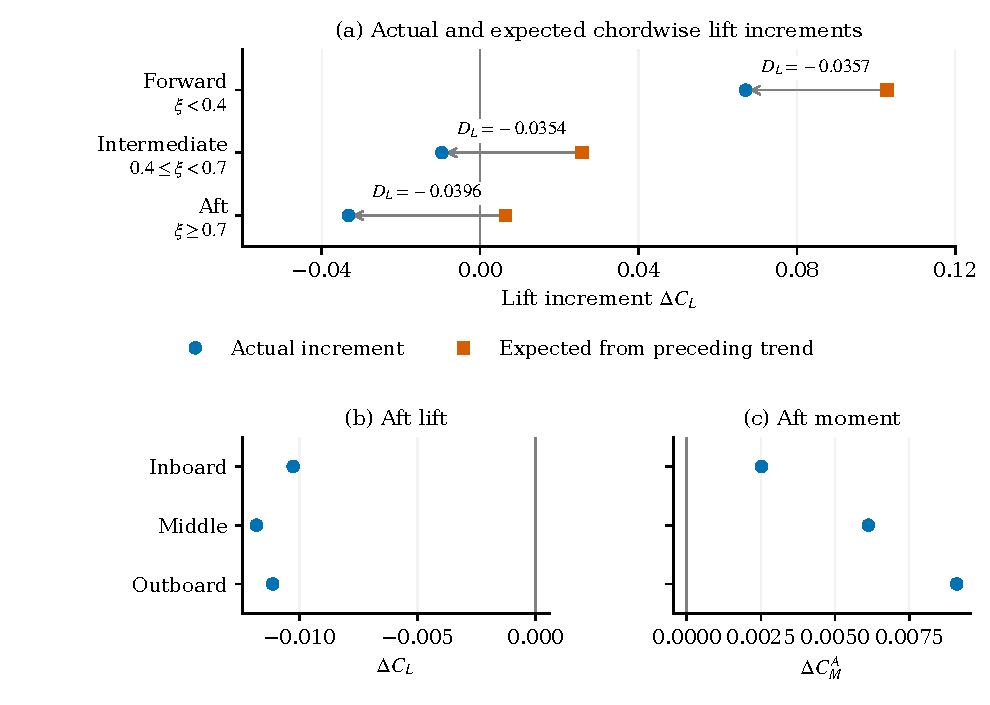
\includegraphics[width=\textwidth]{figures_revision_spatial_changes.pdf}
\caption{Chordwise and spanwise contributions to reference lift and pitching-moment changes over the selected pre-stall interval.}\label{fig:spatial}\end{figure}

The spanwise breakdown shows how the computed lift and moment change from $\alpha=0\degc$ to $2\degc$. From root to tip, the aft thirds contribute similar decreases in lift coefficient ($-0.0103$, $-0.0118$, and $-0.0111$). The nose-up moment increments grow toward the tip ($+0.00252$, $+0.00612$, and $+0.00910$, Fig.~\ref{fig:spatial}b,c). The aft-swept planform places the outboard loads farther behind the computed aerodynamic center. A reduction in upward force behind that axis produces a nose-up moment change, and the same force reduction produces a larger change farther behind the axis. This is the $-(x-x_A)dF_z$ contribution in Eq.~\ref{eq:moment}. The axial-force term $z\,dF_x$ is small in this case.
\label{end:sec:pressure}
\subsection{Skin friction and reverse flow}\label{sec:reversal}
As the aft region loses lift from $\alpha=0\degc$ to $2\degc$, the area of reverse flow on the upper control surface grows (Fig.~\ref{fig:reversal}).

\begin{figure}[htbp]\centering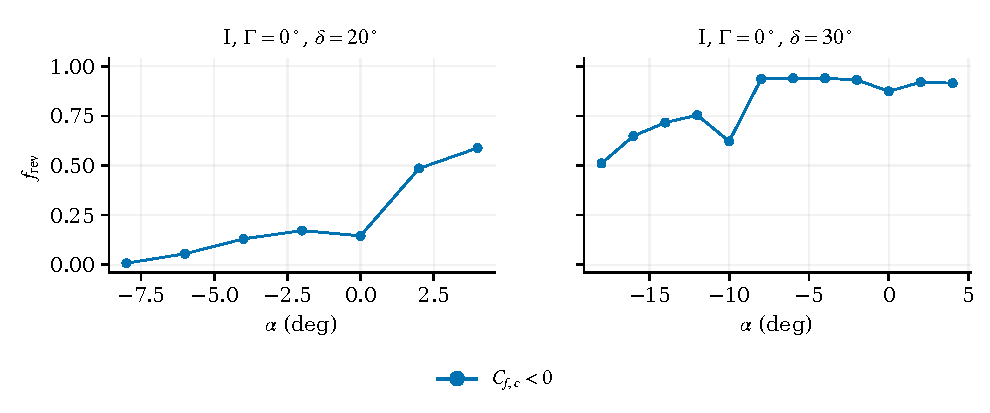
\includegraphics[width=.90\textwidth]{figures_revision_reversal.pdf}
\caption{Reference zero-dihedral upper control surface area fraction with reverse flow at $\delta=20\degc$ and $\delta=30\degc$.}\label{fig:reversal}\end{figure}

At $\delta=20\degc$, the reverse-flow area fraction rises from 0.146 to 0.485 across $\alpha=0\to2\degc$, coinciding with the computed lift-growth shortfall and positive moment change. Figure~\ref{fig:transition} shows that the reversed-shear region also changes location.

At zero incidence, the reverse flow near the wall lies chiefly near the hinge. At $\alpha=2\degc$ it is concentrated toward the trailing edge, then extends upstream by $\alpha=4\degc$ (Fig.~\ref{fig:transition}). From $\alpha=0\degc$ to $2\degc$, suction near the hinge weakens and the aft region loses lift.

By $\alpha=4\degc$, about 59\% of the upper control surface has upstream-directed chordwise shear. Even as this area grows, the model gains more lift from $\alpha=2\degc$ to $4\degc$ (0.0968 in lift coefficient) than from $0\degc$ to $2\degc$ (0.0242).

\begin{figure}[htbp]\centering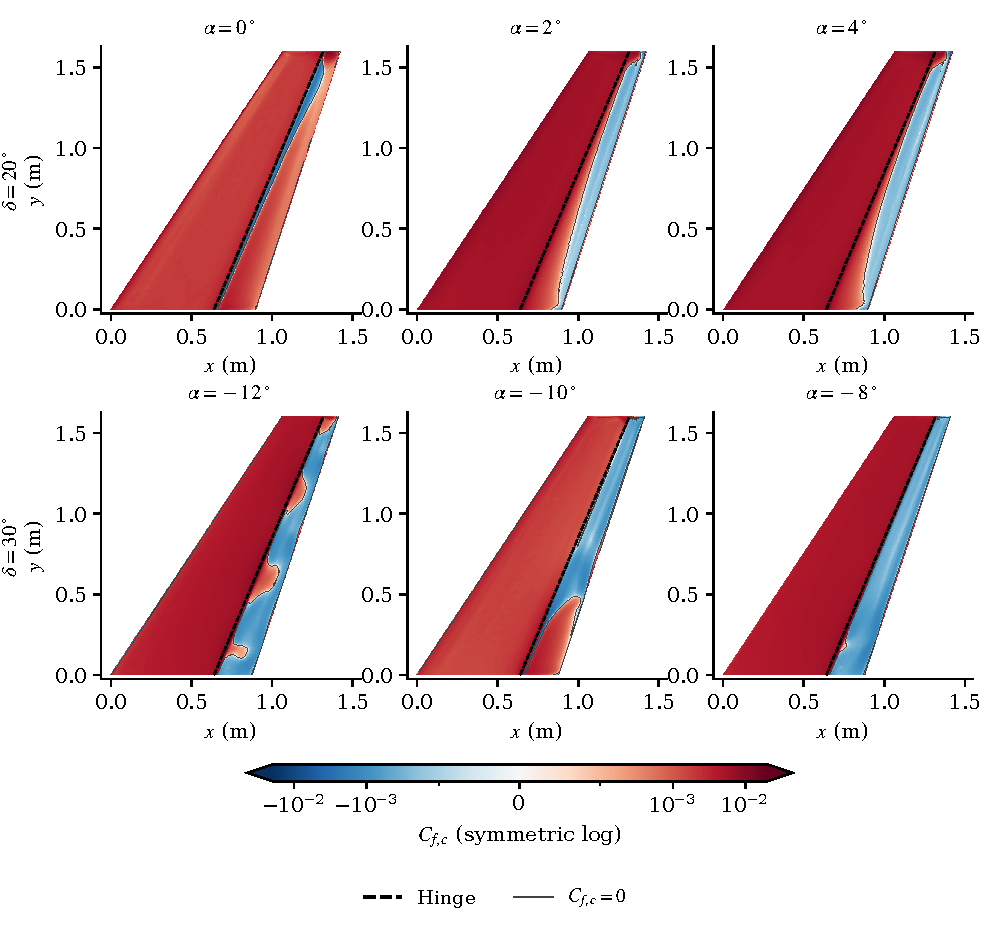
\includegraphics[width=\textwidth]{figures_revision_surface_sequence.pdf}
\caption{Reference upper-surface chordwise skin friction across the loading changes at $\delta=20\degc$ (top) and $\delta=30\degc$ (bottom) deflection.}\label{fig:transition}\end{figure}

At $\delta=30\degc$, the computed loading change occurs at lower incidence, from $\alpha=-10\degc$ to $-8\degc$. The fixed-surface lift coefficient rises by 0.0406, and the control contribution falls by 0.0436, so the total falls by 0.0030. The area fraction with reverse flow rises from 0.622 to 0.935 over this interval (lower row of Fig.~\ref{fig:transition}).

Over the same interval at $\delta=30\degc$, the fixed-surface moment departure is negative and the control moment departure is positive. The total moment departure ranges from $-0.0262$ to $+0.0076$ across the tested fitting ranges. The lift and moment results at the two deflections show why the area with reverse flow needs to be read alongside the pressure and load distributions.
\FloatBarrier
\label{end:sec:joint}
\label{end:sec:reversal}
\section{Dihedral and Planform Dependence}\label{sec:geometry_effects}
We next compare where and by how much lift growth slows across dihedral settings and planforms. We also compare the accompanying pitching-moment changes. The computed load breakdown shows how the fixed surface and control contribute to these differences.

Table~\ref{tab:wt_geometry} gives the measured departures and uncertainty sensitivities for these cases. The primary fits use $\alpha=-6,-4,-2\degc$ at $\delta=20\degc$ and $\alpha=-8,-6,-4\degc$ at $\delta=30\degc$.

\begin{table}[htbp]\centering\small
\caption{Measured lift and moment departures and uncertainty sensitivities for the dihedral and forward-swept cases}\label{tab:wt_geometry}
\begin{tabular}{llrrrr}\toprule
Geom., $\Gamma$, $\delta$ & Coefficient & $\alpha$ interval (deg) & $D$ & $u_{\mathrm{ind}}$ & $u_{\mathrm{L1}}$ \\\midrule
\tablerows{tables_revision_wt_geometry_rows}
\bottomrule\end{tabular}\end{table}

\subsection{Effect of dihedral}\label{sec:dihedral}
Figure~\ref{fig:comparison_dihedral} compares the measurements at the two dihedral settings and the RANS results at $\Gamma=45\degc$. Shading marks the measured intervals in Table~\ref{tab:wt_geometry}. Both deflections share the shaded lift interval. On the moment plots, plain and hatched shading denote $20\degc$ and $30\degc$, respectively. On the 45-degree model at $\delta=20\degc$, the lift curve flattens from $\alpha=-2\degc$ to $2\degc$. The magnitude of the moment departure from $-2\degc$ to $0\degc$ is below both uncertainty sensitivities in Table~\ref{tab:wt_geometry}. At $\delta=30\degc$, measured lift growth slows from $\alpha=-2\degc$ to $0\degc$. The moment coefficient falls by 0.027 in the preceding interval, from $\alpha=-4\degc$ to $-2\degc$. The magnitude of that moment departure exceeds the sensitivity based on independent errors and lies within the absolute-weight bound.

\begin{figure}[htbp]\centering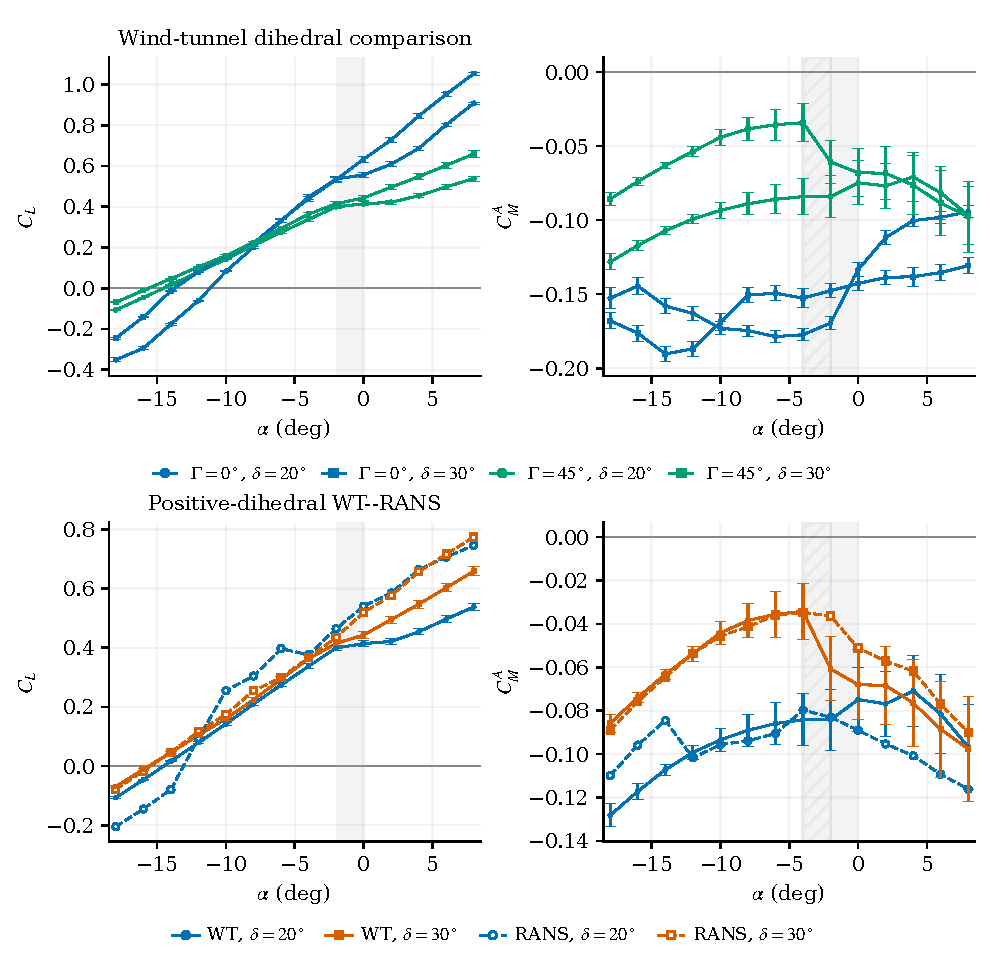
\includegraphics[width=\textwidth]{figures_revision_comparison_dihedral.pdf}
\caption{Dihedral WT and RANS comparisons. Error bars show propagated WT uncertainties.}\label{fig:comparison_dihedral}\end{figure}

At $45\degc$ dihedral and $\delta=20\degc$, RANS predicts a lift decrease from $\alpha=-6\degc$ to $-4\degc$ that is absent in the measurements. In the computation, the area of reverse flow on the control increases markedly over those two degrees. Near the measured reduction in lift growth, the computed lift coefficient rises by 0.0763 over $\alpha=-2\to0\degc$ and by 0.0444 over the next two degrees. At $\delta=30\degc$, the computed moment falls one incidence interval higher than in the tunnel. We use the calculations below to distinguish how dihedral changes the lift increments and which forces contribute to the computed pitching moment.

At zero incidence and $\delta=20\degc$, the computed $C_L$ is 0.301 lower with $45\degc$ dihedral. Tilting the zero-dihedral panel-normal force through $45\degc$ while holding its magnitude fixed would reduce $C_L$ by 0.247.

The effect on lift growth depends on incidence. At $\delta=20\degc$, the zero-dihedral model gains more lift from $\alpha=-2\degc$ to $0\degc$ (0.1210 versus 0.0763 in lift coefficient). From $\alpha=0\degc$ to $2\degc$, the $45\degc$ model gains more (0.0444 versus 0.0242). Its lift coefficient remains lower at both endpoints. In this second interval, the fixed surface of the $45\degc$ model gains lift and the control loses lift. Evaluated about that model's computed aerodynamic center, the fixed surface, control, and tip each contribute to the decrease in pitching moment (Table~\ref{tab:geometry_budget}).

\begin{table}[htbp]\centering\small
\caption{Computed lift and moment increments by surface for the dihedral and forward-swept cases}\label{tab:geometry_budget}
\begin{tabular}{llrrrr}\toprule
Geom., $\Gamma$, $\delta$, $\alpha$ interval & Increment & Fixed & Control & Tip & Total \\\midrule
\tablerows{tables_revision_geometry_budget_rows}
\bottomrule\end{tabular}\end{table}

Table~\ref{tab:geometry_budget} gives the surface contributions to pitching moment about each model's own computed aerodynamic center. Figure~\ref{fig:dihedral} evaluates both models about $A_I$ to compare their moment changes about the same axis~\cite{maggin1946dihedral}. The panels show $\delta=20\degc$ and $30\degc$ from left to right. Dihedral changes the height $z$ at which the axial force acts and hence its moment, $z\,dF_x$. The moment of the upward force is $-(x-x_A)dF_z$, where $x-x_A$ is positive downstream of the axis. For the same incidence interval, we subtract the zero-dihedral moment increment from the 45-degree increment
\begin{equation}
 \mathcal I_M=[C_{M,45}^{A_I}(\alpha_b)-C_{M,45}^{A_I}(\alpha_a)]
             -[C_{M,0}^{A_I}(\alpha_b)-C_{M,0}^{A_I}(\alpha_a)]
\label{eq:interval}
\end{equation}
When $\mathcal I_M$ is negative, the pitching-moment coefficient increases less or decreases more at $45\degc$ than at zero dihedral over the same interval.

\begin{figure}[htbp]\centering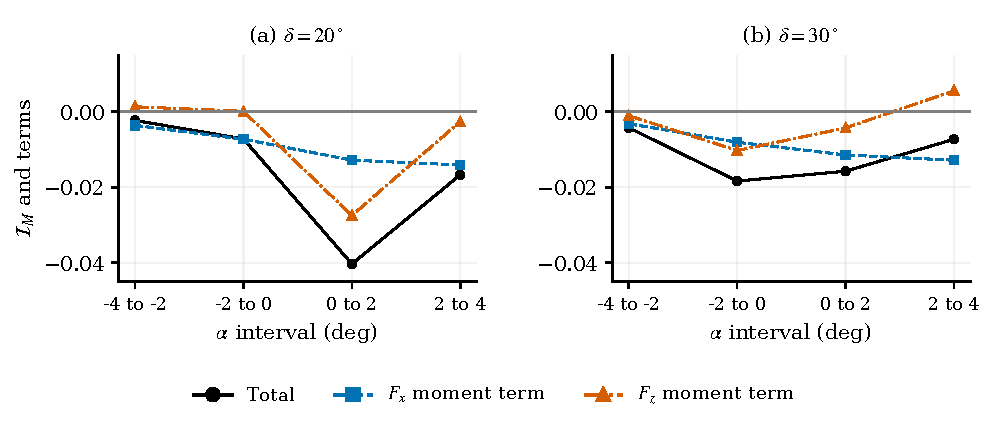
\includegraphics[width=\textwidth]{figures_revision_dihedral_intervals.pdf}
\caption{Difference in pitching-moment increments between $45\degc$ and zero dihedral about $A_I$, with axial and upward force contributions.}\label{fig:dihedral}\end{figure}

At $\delta=20\degc$, the $F_x$ and $F_z$ contributions to the common-axis difference partly cancel over $\alpha=-4\to-2\degc$ ($-0.00362$ and $+0.00131$). Over $\alpha=0\to2\degc$, both are negative ($-0.01283$ and $-0.02750$), giving a total difference of $-0.04033$. The contribution from the upward force is larger in this interval. It depends on how the upward force changes across the surface and on the streamwise distance of each region from the reference axis (Fig.~\ref{fig:dihedral}).

At $\delta=30\degc$, both terms are negative from $\alpha=-2\degc$ to $0\degc$. About the common axis, the moment increment for the $45\degc$ model is therefore 0.01836 lower than for the zero-dihedral model.

For the $45\degc$ model alone, we evaluate the moment about its own computed aerodynamic center. At $\delta=30\degc$, this moment coefficient falls by 0.0148 as $\alpha$ rises from $-2\degc$ to $0\degc$. The fixed surface contributes $-0.0112$ of that change (Table~\ref{tab:geometry_budget}). The area fraction with reverse flow on the control changes only from 0.889 to 0.911 and is 0.912 at $\alpha=2\degc$ (Fig.~\ref{fig:reversal_geometry}). The fixed surface supplies most of the moment change. We therefore examine how its pressure and wall shear vary across the same incidence range.

\begin{figure}[htbp]\centering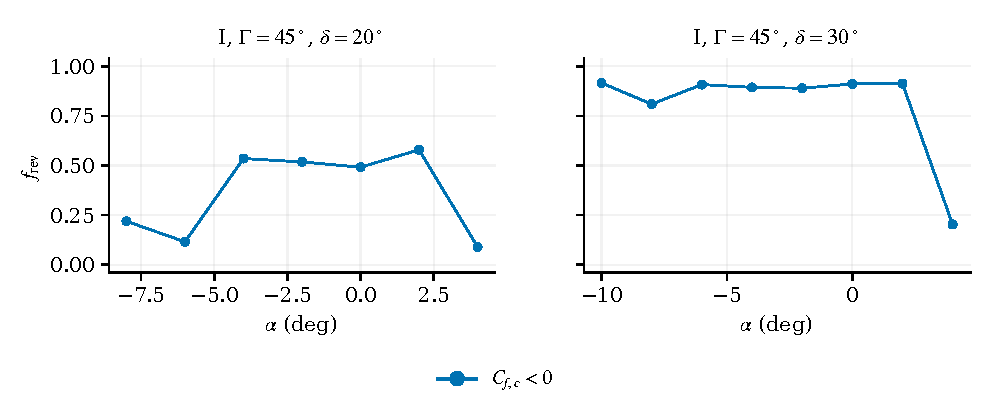
\includegraphics[width=.90\textwidth]{figures_revision_reversal_geometry.pdf}
\caption{Reverse-flow area fractions on the upper control surface for $\Gamma=45\degc$ at $\delta=20\degc$ and $\delta=30\degc$.}\label{fig:reversal_geometry}\end{figure}

From $\alpha=-2\degc$ to $0\degc$, chordwise skin friction increases over the fixed surface from midspan toward the tip (Fig.~\ref{fig:flow_dihedral}). At $\alpha=2\degc$, upstream-directed shear appears near the outboard leading edge. The chordwise cut shows that shear points downstream again farther aft and rises sharply. Together with the localized suction peaks, this pattern is consistent with local separation followed by reattachment.

\begin{figure}[htbp]\centering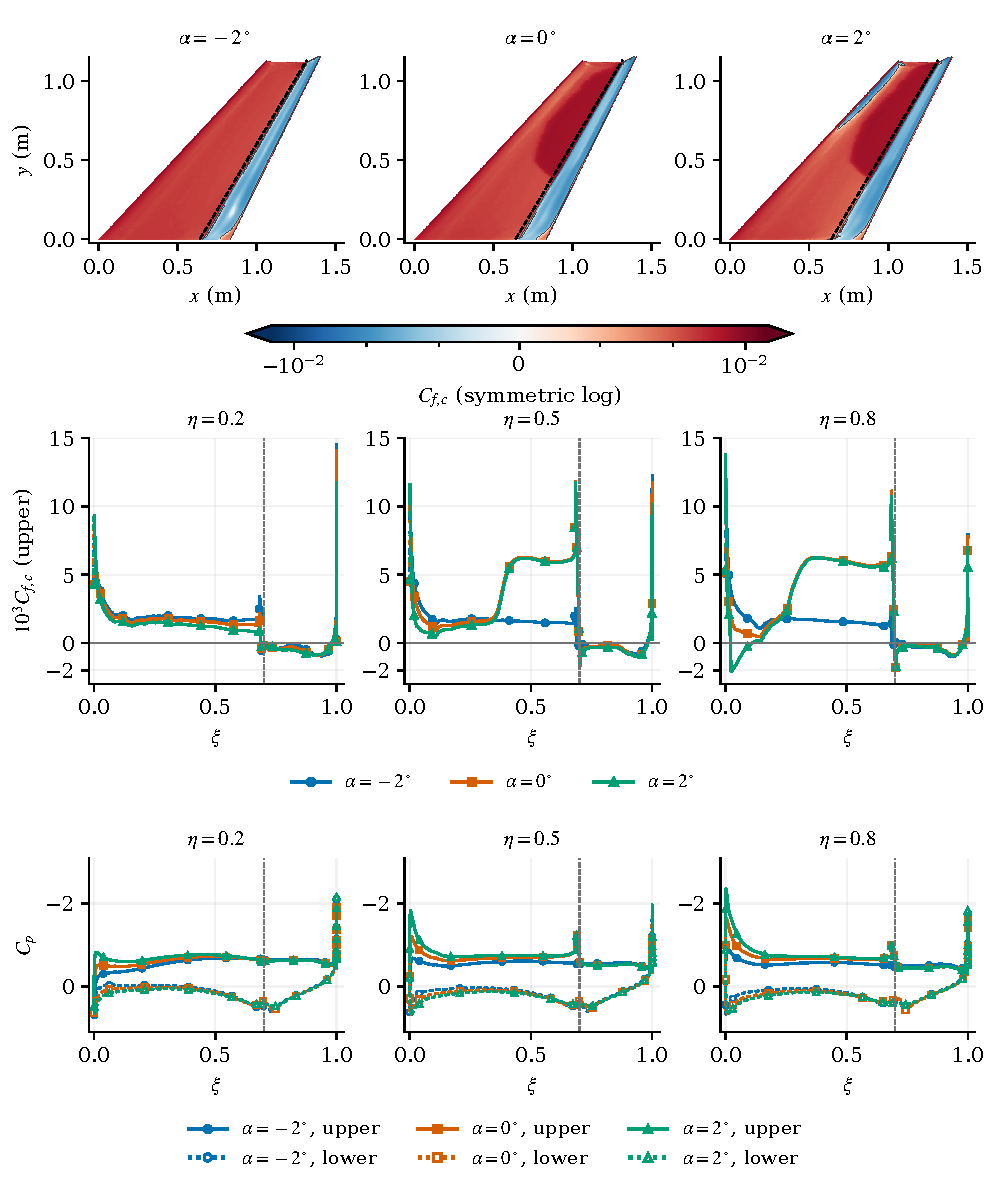
\includegraphics[width=\textwidth]{figures_revision_flow_dihedral.pdf}
\caption{$\Gamma=45\degc$, $\delta=30\degc$: upper-surface shear maps (top), upper-surface shear cuts (middle), and pressure sections (bottom) at $\alpha=-2,0,2\degc$.}\label{fig:flow_dihedral}\end{figure}

At zero incidence, the pressure cuts show stronger leading-edge and hinge suction at midspan and outboard than inboard.

The control pressure changes little over most of its chord from $\alpha=-2\degc$ to $2\degc$, while the fixed-surface pressure and shear change appreciably. These distributions are consistent with the larger fixed-surface contribution to the computed moment decrease from $-2\degc$ to $0\degc$.

\label{anchor:saved_state}Figure~\ref{fig:reversal_geometry} also shows a sharp change at higher incidence. Between $\alpha=2\degc$ and $4\degc$ on the $45\degc$ model, the computed area fraction with reverse flow on the upper control falls from about 0.58 to 0.09 at $\delta=20\degc$ and from 0.91 to 0.20 at $\delta=30\degc$. The reason for these sharp decreases remains unresolved.
\FloatBarrier
\label{end:sec:dihedral}

\subsection{Aft- and Forward-Swept Planforms}\label{sec:planform}
Quarter-chord sweep is $-15\degc$ on model II and $+30\degc$ on model I. Both models have the same semispan and a full-span control. They also differ in taper, chord, and area (Table~\ref{tab:geometry}).

At $\delta=20\degc$, the wind-tunnel lift coefficient of model II rises by 0.044 from $\alpha=0\degc$ to $2\degc$, compared with about 0.092 over each neighboring two-degree interval. The moment coefficient rises by 0.019 over $0\degc$ to $2\degc$ (Fig.~\ref{fig:comparison_planform}). The measured lift growth slows one incidence interval higher than on model I, and the accompanying moment rise is smaller. The primary fit gives a moment departure of $+0.0167$, above its absolute-weight bound of 0.0142 (Table~\ref{tab:wt_geometry}). Fitting $\alpha=-4,-2,0\degc$ gives a departure of $+0.0107$, within the corresponding bound of 0.0148. At $\delta=30\degc$, model II does not show the broad reduction in lift growth at the same negative incidences as model I.

\begin{figure}[htbp]\centering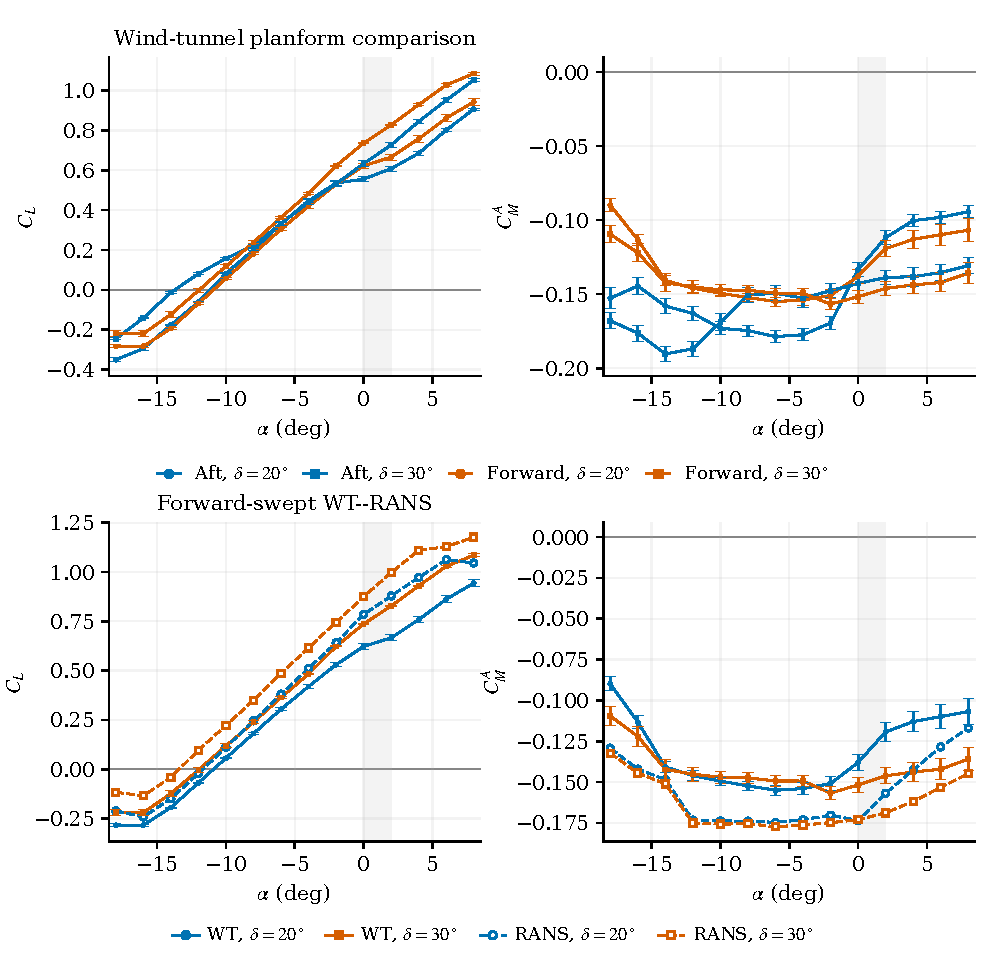
\includegraphics[width=\textwidth]{figures_revision_comparison_planform.pdf}
\caption{Wind-tunnel planform and forward-swept WT--RANS comparisons. WT bars show propagated pointwise uncertainties; grey bands mark the measured $\delta=20\degc$ interval.}\label{fig:comparison_planform}\end{figure}

For the same $0\degc$ to $2\degc$ interval at $\delta=20\degc$, RANS predicts a lift increase of 0.0935, compared with the measured 0.044. The computed moment coefficient rises by 0.0168 about the RANS aerodynamic center. Recalculating that increment about the experimental aerodynamic center gives 0.0099 (Eq.~\ref{eq:transport}, with $\Delta C_{F,z}=0.0952$). About this common axis, RANS therefore predicts about half the measured increase of 0.019.

Figure~\ref{fig:planform_loading} compares the computed load changes on the two zero-dihedral planforms from $\alpha=0\degc$ to $2\degc$ at $\delta=20\degc$. Each moment is evaluated about the corresponding computed aerodynamic center. The coefficients use each model's reference area and chord. The lift coefficient rises more on model II than on model I (0.0935 versus 0.0242). Model II gains more lift on the fixed surface and loses less on the control. The intermediate region gains lift on model II and loses lift on model I, while the loss over the aft region is smaller on model II. The nose-up moment increase is smaller on model II.

\begin{figure}[htbp]\centering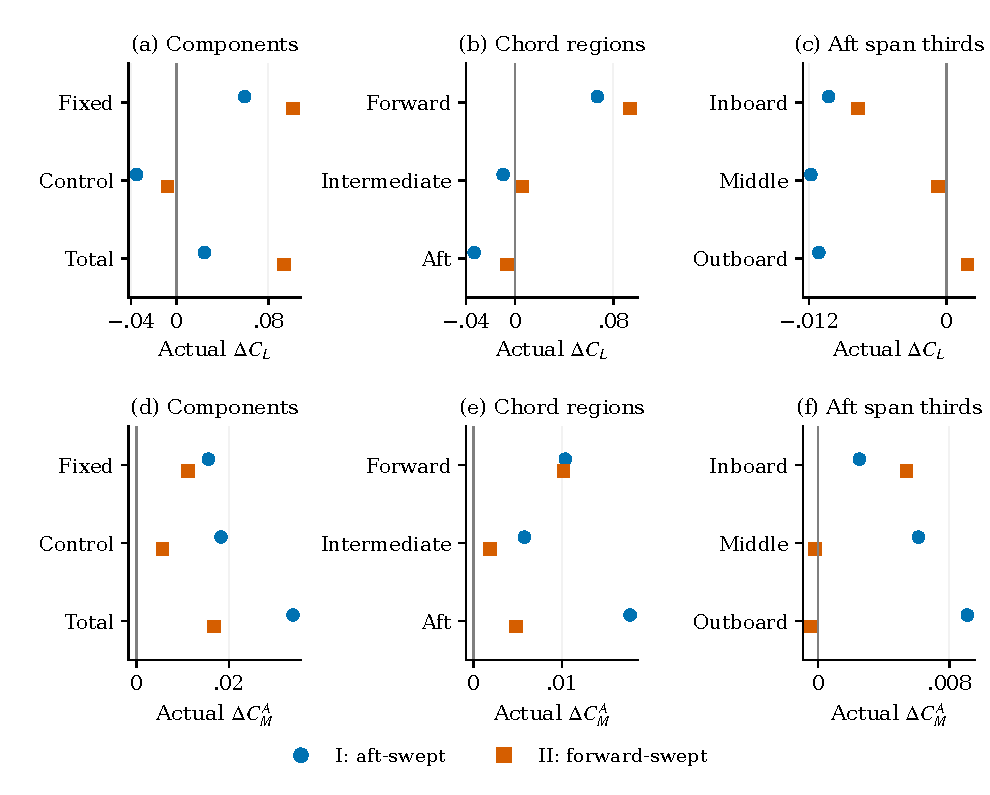
\includegraphics[width=\textwidth]{figures_revision_planform_loading.pdf}
\caption{Planform comparison over $\alpha=0\to2\degc$ at $\delta=20\degc$. Lift increments (top) and moment increments about each model's computed aerodynamic center (bottom).}\label{fig:planform_loading}\end{figure}

\begin{figure}[!tp]\centering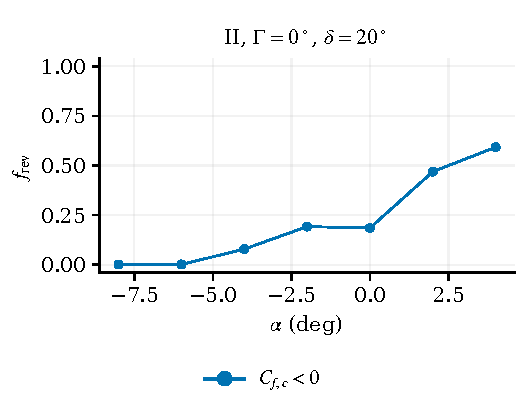
\includegraphics[width=.50\textwidth]{figures_revision_reversal_planform.pdf}
\caption{Upper-control reverse-flow fraction on the forward-swept planform at $\delta=20\degc$.}\label{fig:reversal_planform}\end{figure}

Although model II gains more total lift than model I over this interval, the lift changes on its fixed surface and control are both smaller than their earlier slopes would suggest. Their departures are $-0.0263$ and $-0.0104$, compared with $-0.0692$ and $-0.0414$ on model I. For both models, the fixed-surface and control moment departures are positive when evaluated about the model's computed aerodynamic center. About the original numerical origin of model II, the fixed-surface and control departures are $-0.0023$ and $+0.0035$ and partly cancel.

The moments depend on both the spanwise distribution of the loads and their distance behind the reference axis. On model I, similar aft lift losses along the span produce progressively larger nose-up moment increments toward the tip, where the aft loads act farther behind the axis. On model II, the downstream moment arm decreases toward the tip. As the angle of attack increases over the same interval, the aft region loses lift inboard and gains lift outboard. The nose-up contribution is concentrated inboard. This helps explain why the computed moment increment for model II is about half that of model I despite its larger lift increment. McCormack and Cook~\cite{mccormack1949sweptforward} also linked inboard pressure changes to pitching moment on a forward-swept wing without a control surface.

On model II, the upper-control area fraction with reverse flow rises from about 19\% at zero incidence to 47\% at $\alpha=2\degc$ and 59\% at $4\degc$ (Fig.~\ref{fig:reversal_planform}). The maps show the region spreading upstream and toward the root (Fig.~\ref{fig:flow_planform}). From $\alpha=0\degc$ to $2\degc$, suction near the hinge weakens inboard and changes little outboard, consistent with the aft lift loss being concentrated inboard.

\begin{figure}[!tp]\centering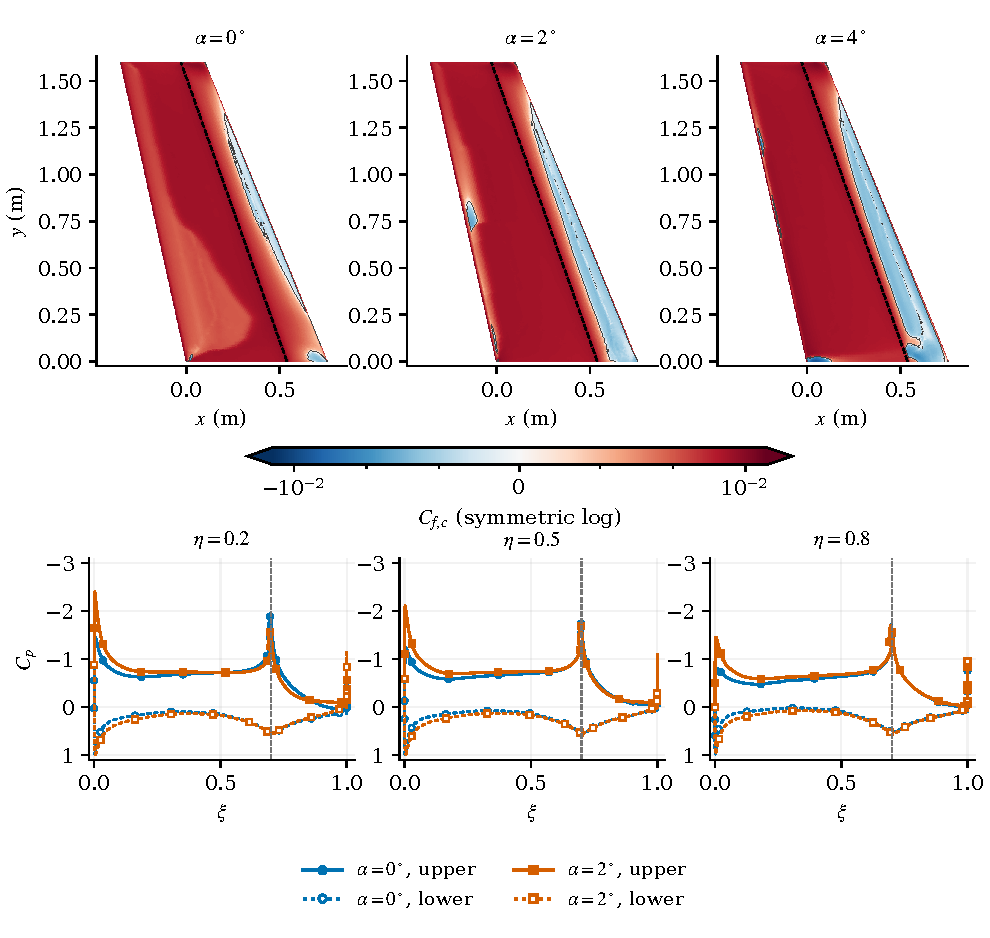
\includegraphics[width=.90\textwidth]{figures_revision_flow_planform.pdf}
\caption{Forward-swept planform, $\delta=20\degc$: upper-surface chordwise shear (top) and pressure sections across $\alpha=0\to2\degc$ (bottom).}\label{fig:flow_planform}\end{figure}

At $\alpha=2\degc$, reverse flow covers a similar fraction of the upper control surface on the two models (47\% on II and 49\% on I). The different pressure changes along the chord and span account for the different control lift losses.
\label{end:sec:planform}
\FloatBarrier
\label{end:sec:geometry_effects}
\section{Conclusions}\label{sec:conclusions}
On the low-aspect-ratio swept tailplane models with full-span control surfaces, wind-tunnel measurements show that lift growth can slow and then recover well before stall. Increasing the control deflection on the aft-swept reference model shifts the reduction in lift growth to lower incidence. The pitching-moment coefficient can depart from its earlier trend over a different interval. At $20\degc$ deflection, RANS places the reduction in lift growth one sampled incidence interval higher than in the experimental results. The computed surface loads show how the lift and moment responses arise.

In the reference calculation at $20\degc$ deflection, total lift grows more slowly from $0\degc$ to $2\degc$ than its preceding trend predicts. The fixed surface gains lift over this interval, but its gain falls below its own fitted trend. That difference accounts for about 63\% of the shortfall in total lift growth. The control loses lift and supplies most of the positive pitching-moment departure about the computed aerodynamic center. Stronger leading-edge suction coexists with lift loss farther aft, and lift growth subsequently recovers while reverse flow continues to spread over the control. The pressure distributions and regional loads thus explain changes that the extent of reverse flow alone cannot describe.

The geometry comparisons show how this response varies with incidence. At $20\degc$ control deflection, dihedral reduces the computed lift gain over the interval just below zero incidence and increases it over the next interval. Both axial and upward forces contribute to the corresponding moment differences about a common axis. In the experimental results, the reduction in lift growth occurs at a higher incidence for the forward-swept planform than for the aft-swept reference. From $0\degc$ to $2\degc$, the forward-swept model has a smaller computed lift-growth shortfall. Its nose-up moment increment is also smaller when the moments are evaluated about each model's computed aerodynamic center. Its aft lift loss is concentrated inboard, while on the aft-swept model the loss extends outboard, where it acts through longer moment arms. The changes in lift growth and pitching moment together show how the pre-stall response depends on both the strength and location of the load changes.

Future work will assess how the wind-tunnel boundary layer over the raised floor affects the pre-stall response. Higher-fidelity hybrid RANS--LES simulations will also be used to test whether they improve agreement with the measured lift and pitching moment.
\appendix
\label{end:sec:conclusions}
\section{Sensitivity Checks}\label{app:sensitivity}
We check how the earlier fit, the choice of surface regions, and the wall-shear threshold affect the reported quantities.

Table~\ref{tab:sensitivity} compares the reference departures from $\alpha=0\degc$ to $2\degc$ at $\delta=20\degc$, with moments about the computed aerodynamic center. Across the three fits, the fixed-surface share of the reference lift-growth shortfall stays between 62.4\% and 62.6\%. The total lift departure is more sensitive to the choice of fit, ranging from $-0.137$ to $-0.105$.

\begin{table}[htbp]\centering\small
\caption{Sensitivity of reference lift and pitching-moment departures to the fitted incidence range}\label{tab:sensitivity}
\begin{tabular}{lrrr}\toprule
Preceding $\alpha$ (deg) & Total $D_L$ & Fixed fraction (\%) & Total $D_M$ \\\midrule
\tablerows{tables_revision_sensitivity_rows}
\bottomrule\end{tabular}\end{table}

Figure~\ref{fig:partition_check} compares spanwise-third and spanwise-quarter partitions, with alternative chord subdivisions.

\begin{figure}[htbp]\centering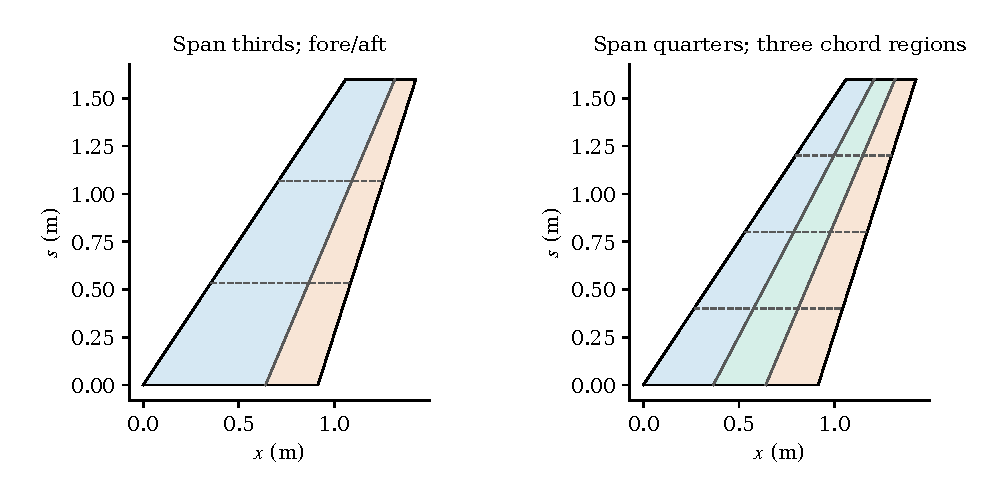
\includegraphics[width=.80\textwidth]{figures_revision_partition_check.pdf}
\caption{Alternative integration partitions: spanwise thirds with fore/aft regions (left), and quarters with forward/intermediate/aft regions (right).}\label{fig:partition_check}\end{figure}
\FloatBarrier

Narrowing the inboard region from one-third to one-quarter of the semispan changes the aft lift departure from $-0.0127$ to $-0.00939$. It remains negative. Dividing the fixed chord more finely also leaves both fixed-region lift departures negative.

The main text compares chordwise and spanwise load changes with the extent of upstream-directed near-wall shear on the control. Replacing the zero threshold with small negative values, $C_{f,c}<-10^{-6}$ and $C_{f,c}<-10^{-5}$, leaves the reference result nearly unchanged. With the more negative cutoff, the $\delta=20\degc$ fraction grows from 0.145 to 0.480 across $\alpha=0\to2\degc$, compared with 0.146 to 0.485 in Fig.~\ref{fig:reversal}.

\label{end:app:sensitivity}
\FloatBarrier
\section*{Acknowledgments}\label{anchor:acknowledgments}
This project has received funding from the Clean Sky 2 Joint Undertaking (JU) under grant agreement No 101008257. The JU receives support from the European Union's Horizon 2020 research and innovation programme and the Clean Sky 2 JU members other than the Union.

The authors used generative artificial intelligence tools (Claude, Anthropic, and Codex, OpenAI) to assist in writing the scripts that post-processed the existing wind-tunnel and numerical data and produced the figures, and to assist in drafting and editing the text and improving its grammar and correctness. Grammarly was used for grammar and style checks. The wind-tunnel measurements and RANS solutions were obtained independently of these tools. The authors reviewed and verified all scripts, figures, and text, and take full responsibility for the content of this paper.
\label{anchor:references}\bibliography{References}
\label{end:references}
\end{document}
